\documentclass[11pt]{article}

\usepackage[utf8]{inputenc}
\usepackage[T1]{fontenc}
\usepackage[spanish,es-noquoting,es-tabla]{babel}
\usepackage[letterpaper,margin=2.1cm]{geometry}
\usepackage{newtxtext,newtxmath}
\usepackage{booktabs}
\usepackage{graphicx}
% Las figuras se toman de su ubicación versionada, para no duplicarlas aquí.
\graphicspath{{../tesis/images/}}
\usepackage{caption}
\usepackage{enumitem}
\usepackage{xcolor}
\usepackage{mdframed}
\usepackage{titlesec}
\usepackage{float}
\usepackage[hidelinks]{hyperref}
\usepackage{siunitx}
\sisetup{output-decimal-marker={,},group-separator={{.}}}

\definecolor{azul}{HTML}{0B3D91}
\definecolor{rojo}{HTML}{C0392B}
\definecolor{verde}{HTML}{1E6B45}
\definecolor{fondo}{HTML}{F1F5FA}

\titleformat{\section}{\large\bfseries\color{azul}}{\thesection.}{0.6em}{}
\titleformat{\subsection}{\normalsize\bfseries}{\thesubsection}{0.6em}{}
\setlist{nosep, leftmargin=1.3em}
\captionsetup{font=small, labelfont={small,bf}}

\newmdenv[backgroundcolor=fondo, linewidth=0pt, skipabove=5pt, skipbelow=9pt,
          innertopmargin=7pt, innerbottommargin=7pt]{caja}

% Pregunta para la directora, numerada aparte del cuerpo.
\newcounter{preg}
\newcommand{\preg}[1]{\refstepcounter{preg}%
  \medskip\noindent\textbf{\color{rojo}Pregunta \thepreg.}\; \textbf{#1}\par\nopagebreak}

\title{\vspace{-1.6cm}\textbf{Estado del trabajo de grado}\\[2mm]
\large Conteo de rocas visibles basado en las máscaras de AI4Mars\\[3mm]
\normalsize Documento de reunión con la dirección de tesis}
\author{Juan Pablo Delgado Castro}
\date{}

\begin{document}
\maketitle
\thispagestyle{empty}

\begin{caja}
\noindent\textbf{Resumen de la situación.} El documento está redactado y compila:
\textbf{87 páginas} sobre la plantilla oficial del Departamento. Los cinco objetivos
específicos están cumplidos. El procedimiento se ejecutó sobre las \num{16064} escenas del
subconjunto. Se realizó una validación con conteo humano de \num{60} escenas y un contraste
con dos enfoques de aprendizaje automático.

\smallskip
\noindent Traigo \textbf{ocho decisiones} que necesito consultar, listadas en la
sección~\ref{sec:preguntas}. Las dos más importantes son la \textbf{estructura del
documento} (Pregunta~1) y el \textbf{encuadre de los resultados}
(Pregunta~3).
\end{caja}

\section{Qué se hizo}

\subsection{El procedimiento, paso a paso}

Para cada máscara se calculan dos indicadores. La \textbf{cobertura de roca visible} es
directa: el cociente entre los píxeles de roca y los píxeles que la anotación etiquetó.
El \textbf{conteo de rocas} es el problema difícil, porque la máscara no distingue
instancias: si dos rocas se tocan, quedan registradas como una sola región conectada, y
separarlas exige criterios geométricos. Son cinco etapas.

\begin{enumerate}[leftmargin=1.8em]

\item \textbf{Máscara binaria.} De los cinco valores posibles de la máscara se conserva
  solo la clase \textit{roca grande}: queda una imagen de unos y ceros. Todo lo demás
  —suelo, arena, lecho rocoso y los píxeles sin etiquetar— pasa a ser fondo.

\item \textbf{Limpieza morfológica.} Se aplica una \emph{apertura} seguida de un
  \emph{cierre}, ambas con una ventana de $3\times3$ píxeles. La apertura elimina motas
  aisladas, producto de imprecisiones al trazar los polígonos de anotación; el cierre
  rellena huecos pequeños dentro de una misma región. Sin este paso, cada mota contaría
  como candidata a roca.

\item \textbf{Transformada de distancia.} A cada píxel de roca se le asigna
  \textbf{su distancia al borde más cercano}. Los centros de las regiones reciben valores
  altos y los bordes, valores bajos. El resultado se lee como un relieve: cada roca es una
  colina, y \emph{el punto donde dos rocas se tocan es un valle}, porque ahí el borde está
  cerca por ambos lados. Ese valle es la clave de la etapa siguiente.

\item \textbf{División de aguas.} Se sitúan semillas en las cimas de ese relieve y se
  «inunda» desde ellas hasta que las regiones se encuentran. La frontera queda justo en el
  valle, es decir, en el estrangulamiento donde un observador humano también separaría las
  dos rocas. Las semillas se eligen por \textbf{prominencia}: solo se conserva un máximo si
  su altura sobre el entorno supera un umbral. Esa decisión fue la calibración principal
  del trabajo: sin ella, una losa extensa generaba decenas de semillas espurias —se
  observó un caso con \num{142}— y quedaba fragmentada en rocas inexistentes.

\item \textbf{Filtros de tamaño y forma.} Cada región resultante debe superar dos
  criterios para contarse: un \textbf{área mínima} de \num{524} píxeles
  (\SI{0.05}{\percent} de la imagen), que descarta motas, y una \textbf{relación de
  aspecto} no mayor que 5, que descarta bandas muy alargadas —en la práctica, horizontes
  trazados a mano y no bloques.

\end{enumerate}

\begin{caja}
\noindent\textbf{Lo que hay que retener del método.} Los siete umbrales son
\textbf{números explícitos y documentados}, no ajustes ocultos: cada uno se puede discutir
y cambiar, y el documento registra qué efecto tiene. El procedimiento corre en procesador
convencional, sin entrenar ningún modelo y sin conjunto de entrenamiento, y procesa las
\num{16064} escenas en minutos. Esa transparencia es el argumento del método; no su
sofisticación.

\smallskip
\noindent Y una consecuencia que conviene tener presente desde el principio:
\textbf{el procedimiento no abre las imágenes}. Toda su información proviene de la máscara.
Eso responde la pregunta de si harían falta mejores fotografías —no las usa— y a la vez
impone el techo que documenta la sección~\ref{sec:techo-doc}.
\end{caja}

\begin{table}[H]
\centering\small
\begin{tabular}{llp{5.6cm}}
\toprule
\textbf{Parámetro} & \textbf{Valor} & \textbf{Qué ocurre si se cambia}\\
\midrule
Apertura y cierre & $3\times3$ & Mayor: se pierden rocas pequeñas. Menor: entran motas.\\
Suavizado de la distancia & $\sigma = 3{,}0$ & Menor: el contorno irregular genera cimas
  falsas.\\
Prominencia de la semilla & $h = 1{,}0$ & Menor: sobresegmenta. Mayor: fusiona rocas
  distintas.\\
Área mínima & \num{524} px & Mayor: se descartan rocas reales pequeñas.\\
Relación de aspecto & 5 & Mayor: entran bandas del horizonte como si fueran rocas.\\
Conectividad & 8 vecinos & Con 4, dos rocas unidas en diagonal se separarían.\\
\bottomrule
\end{tabular}
\caption{Los umbrales y su efecto. Ninguno está fijado dentro de la lógica de cálculo:
  todos se pasan como argumentos con su valor por defecto documentado.}
\end{table}

La Figura~\ref{fig:pasoapaso} muestra las etapas sobre una escena real.

\begin{figure}[H]
  \centering
  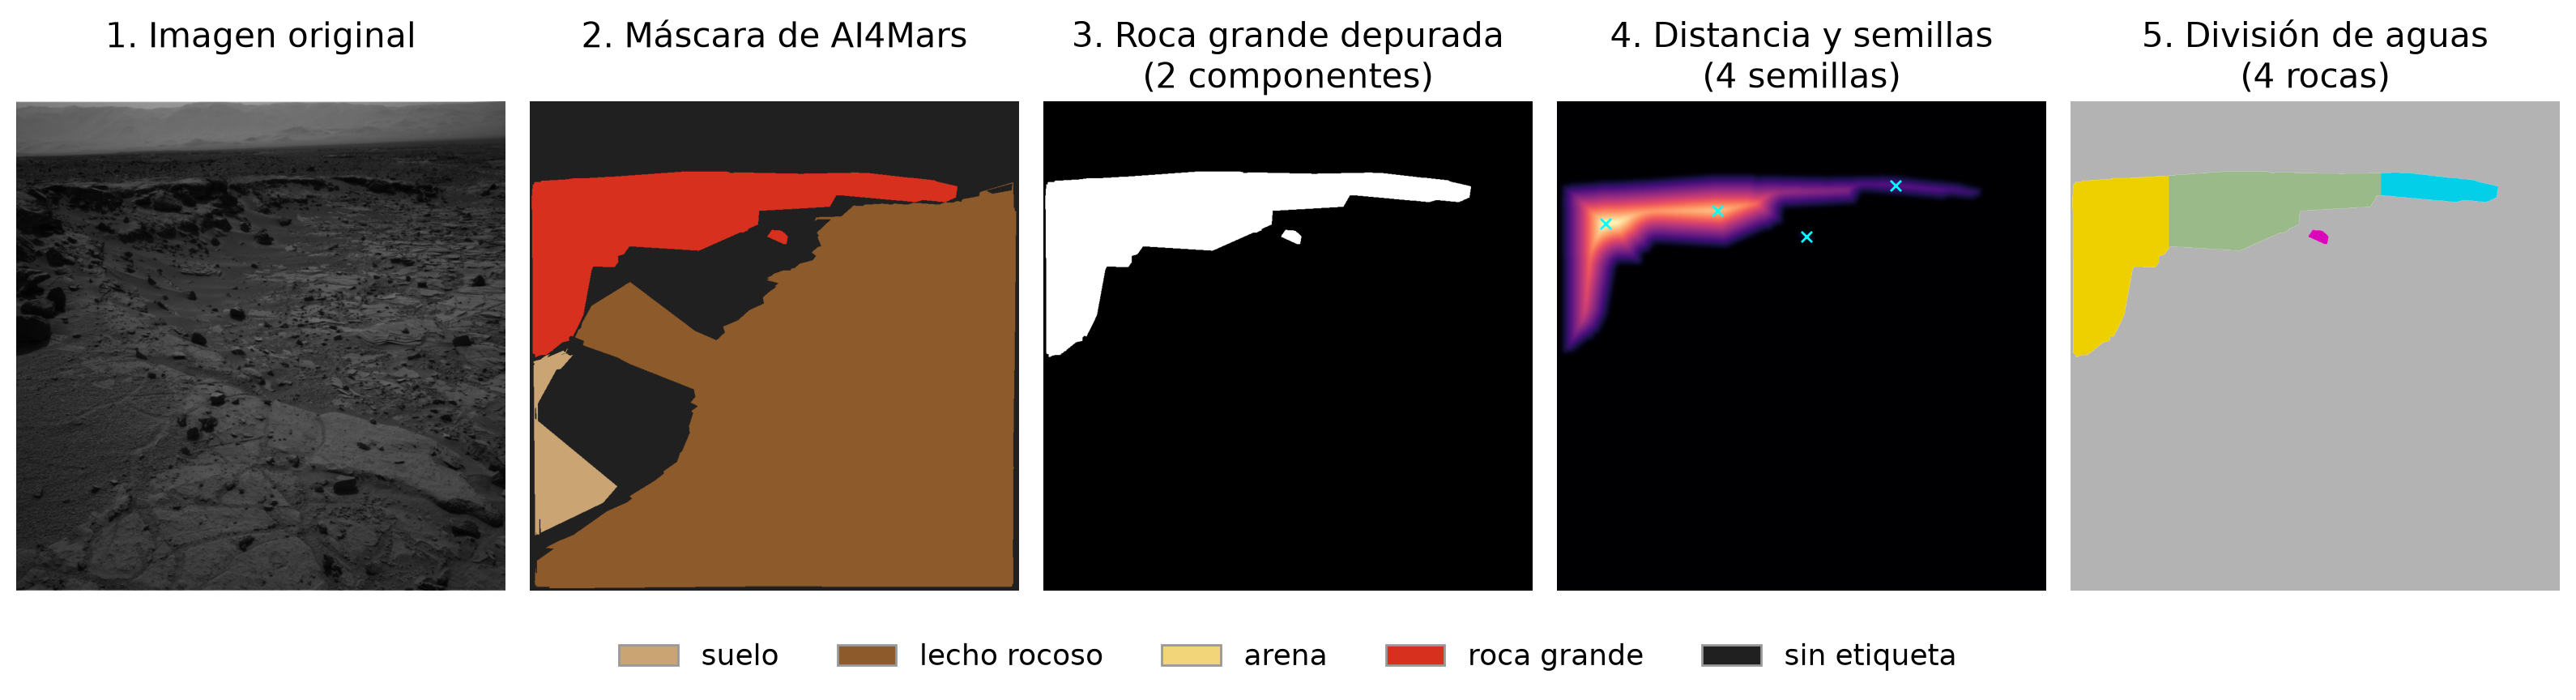
\includegraphics[width=\textwidth]{Figura_11_procedimiento_paso_a_paso.png}
  \caption{Las cinco etapas sobre una escena: imagen original, máscara de AI4Mars, binaria
    depurada, transformada de distancia con las semillas detectadas, y resultado del
    conteo.}
  \label{fig:pasoapaso}
\end{figure}

\subsection{Lo que se entrega}

\begin{itemize}
  \item Archivo de resultados con \textbf{24 indicadores por imagen} para las \num{16064}
    escenas.
  \item Código modular (12 módulos, 22 guiones de ejecución), con parámetros y versiones
    registradas.
  \item 22 figuras y el documento completo en \LaTeX.
  \item Como extensión: un sistema de seis reglas de aviso de terreno y una aplicación de
    escritorio de consulta.
\end{itemize}

\section{Los resultados principales}

\subsection{La cobertura funciona; el conteo tiene un techo}

\begin{table}[H]
\centering\small
\begin{tabular}{lcc}
\toprule
 & \textbf{Cobertura (E1)} & \textbf{Conteo (E2)}\\
\midrule
Escenas donde está definido & \SI{67.3}{\percent} & \SI{13.9}{\percent}\\
Valor central & mediana \SI{96.8}{\percent} & mediana 1 roca\\
Validación & control del denominador ($r=-0{,}02$) & conteo humano ($\kappa = 0{,}13$)\\
\multicolumn{3}{l}{\footnotesize El kappa mide cuánto coincide \emph{el procedimiento} con
el conteo humano, que actúa de referencia.}\\
Veredicto & \textbf{\color{verde}utilizable} & \textbf{\color{rojo}con techo estructural}\\
\bottomrule
\end{tabular}
\caption{Los dos indicadores no están al mismo nivel de solidez, y el documento lo dice.}
\end{table}

Un resultado que no era evidente: los dos indicadores son \textbf{estadísticamente
independientes} ($r = 0{,}02$). Miden cosas distintas —cuánta roca hay y cómo está
organizada— y ninguno sustituye al otro.

\subsection{Hallazgo 1: la anotación colaborativa sobreestima la roca}
\label{sec:sesgo-doc}

El conjunto incluye \num{322} máscaras anotadas por especialistas. Se ejecutó sobre ellas
el mismo código, sin cambiar ningún parámetro.

\begin{table}[H]
\centering\small
\begin{tabular}{lcc}
\toprule
\textbf{Indicador} & \textbf{Colaborativas} & \textbf{Experto}\\
\midrule
Cobertura mediana & \SI{96.8}{\percent} & \textbf{\SI{46.1}{\percent}}\\
Escenas con cobertura total & \SI{41}{\percent} & \textbf{\SI{8}{\percent}}\\
Píxeles de suelo y arena & \SI{50}{\percent} & \textbf{\SI{69}{\percent}}\\
\bottomrule
\end{tabular}
\end{table}

\begin{figure}[H]
  \centering
  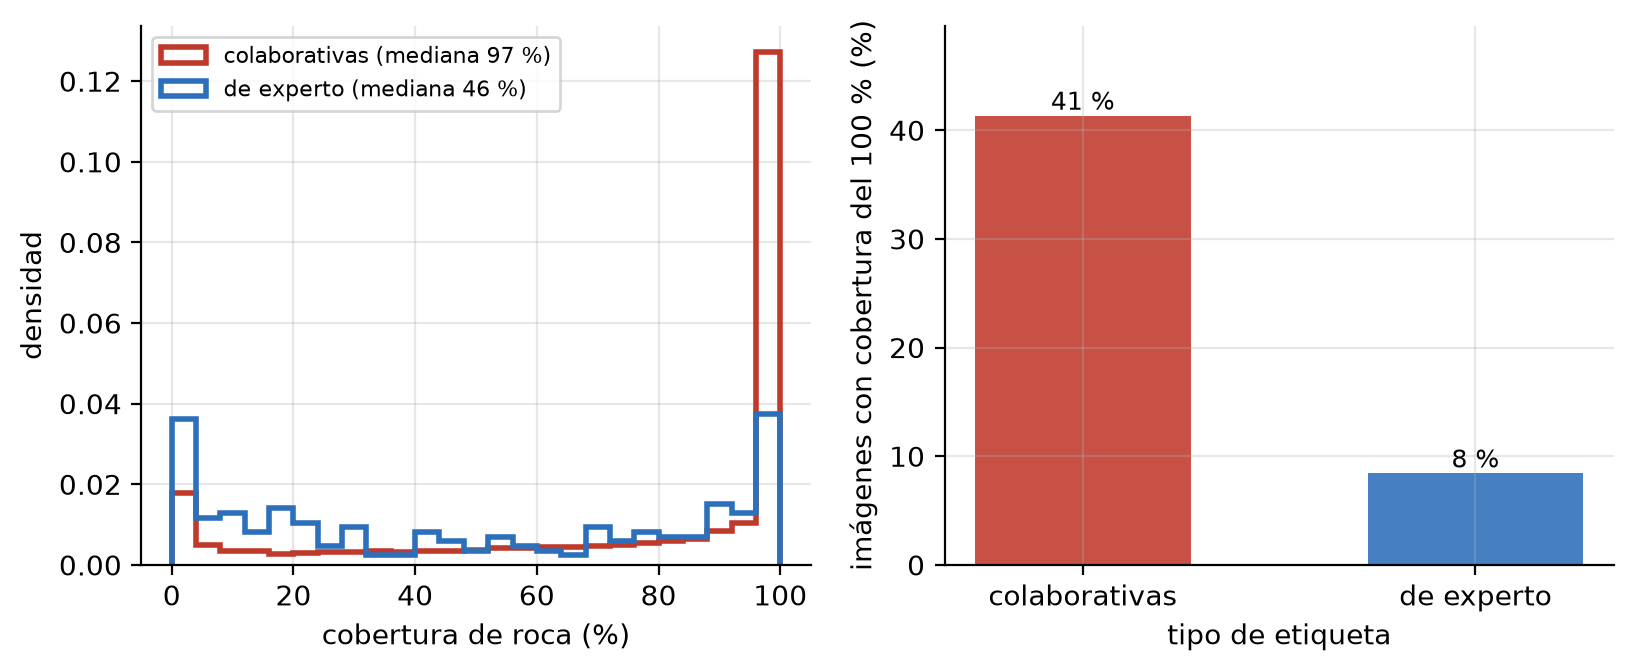
\includegraphics[width=0.72\textwidth]{Figura_19_validacion_experto.png}
  \caption{Comparación de la cobertura entre etiquetas colaborativas y de experto.}
\end{figure}

El mecanismo es un \textbf{sesgo de saliencia}: la roca es visualmente prominente y fácil
de delimitar; el suelo y la arena son superficies extensas cuya anotación es tediosa. Los
píxeles sin consenso quedan sin etiquetar y salen del denominador, lo que eleva la fracción
de roca.

\begin{caja}
\noindent\textbf{Por qué creo que este es el aporte más transferible del trabajo.} Toda la
línea de investigación que usa AI4Mars evalúa sus modelos por el acuerdo con estas
máscaras. Documentar que sobreestiman la roca, y cuantificar cuánto, es información
pertinente para esos trabajos y no solo para el mío.
\end{caja}

\subsection{Hallazgo 2: el techo del conteo es la taxonomía, no las imágenes}
\label{sec:techo-doc}

La explicación intuitiva del bajo desempeño del conteo sería que faltan imágenes mejores.
Se descartó con tres mediciones:

\begin{itemize}
  \item El procedimiento \textbf{no abre las imágenes}: opera solo sobre la máscara. Las
    imágenes ya son de resolución completa (\num{1024}$\times$\num{1024}) y la máscara
    tiene el mismo tamaño.
  \item En \num{13838} escenas (\SI{86.1}{\percent}) la máscara \textbf{no tiene ningún
    píxel} de la clase roca grande. De la roca etiquetada en el conjunto, el lecho rocoso
    aporta el \SI{97.5}{\percent} y la roca grande solo el \SI{2.5}{\percent}.
  \item Las máscaras de experto tienen \textbf{menos} roca grande, no más: del
    \SI{16.5}{\percent} de escenas al \SI{1.6}{\percent} según se endurece el criterio de
    acuerdo.
\end{itemize}

\begin{figure}[H]
  \centering
  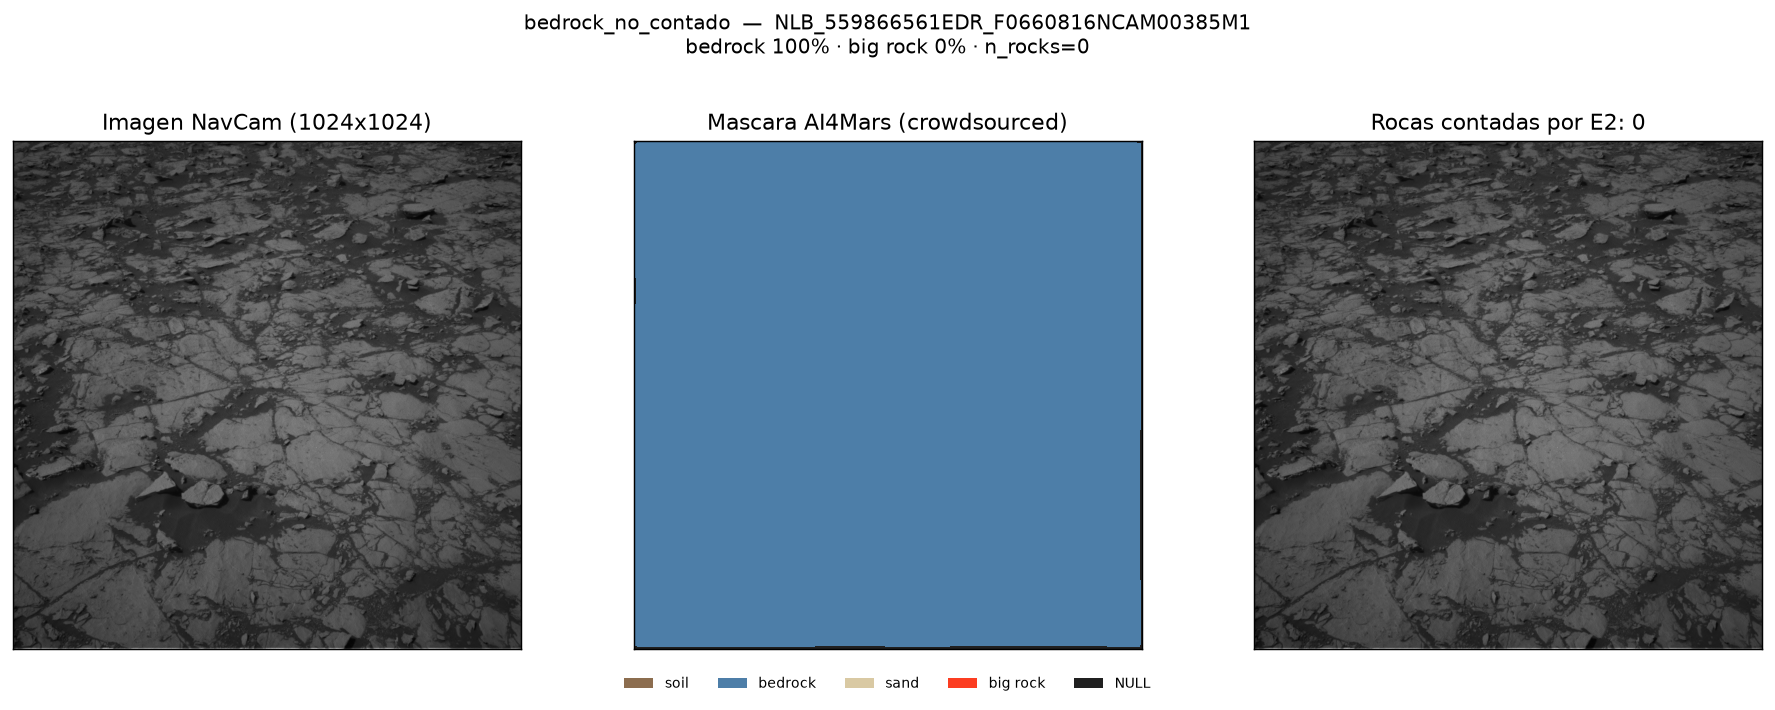
\includegraphics[width=\textwidth]{diag_bedrock_no_contado.png}
  \caption{Escena repleta de bloques individuales evidentes, etiquetada en su totalidad
    como una sola región de lecho rocoso. El conteo devuelve cero. La imagen es excelente;
    la etiqueta es el límite.}
\end{figure}

\subsection{Hallazgo 3: la anotación no es exhaustiva}

La validación con conteo humano lo mostró. En \num{36} de las \num{60} escenas, la clase
roca grande cubre \textbf{menos del \SI{20}{\percent}} de la roca etiquetada, con una
mediana del \SI{9.1}{\percent}: la anotación marca \emph{algunas} rocas, no todas.

\begin{figure}[H]
  \centering
  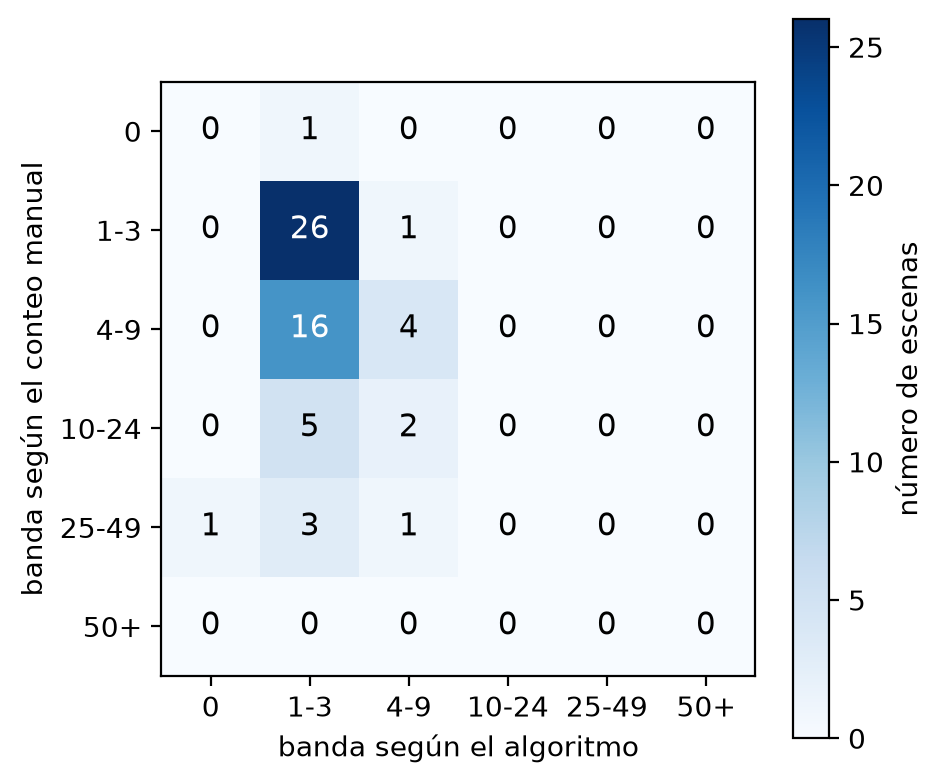
\includegraphics[width=0.66\textwidth]{Figura_26_validacion_manual_v2.png}
  \caption{Acuerdo entre el conteo manual y el automático ($n = 60$). Las tres columnas de
    la derecha están vacías: el procedimiento no supera las nueve rocas en ninguna escena,
    mientras el observador identificó diez o más en doce de ellas.}
\end{figure}

La causa se ve mejor de lo que se explica. La Figura~\ref{fig:mecanismo} contrapone una
escena donde el procedimiento acierta con otra donde subcuenta de forma grave.

\begin{figure}[H]
  \centering
  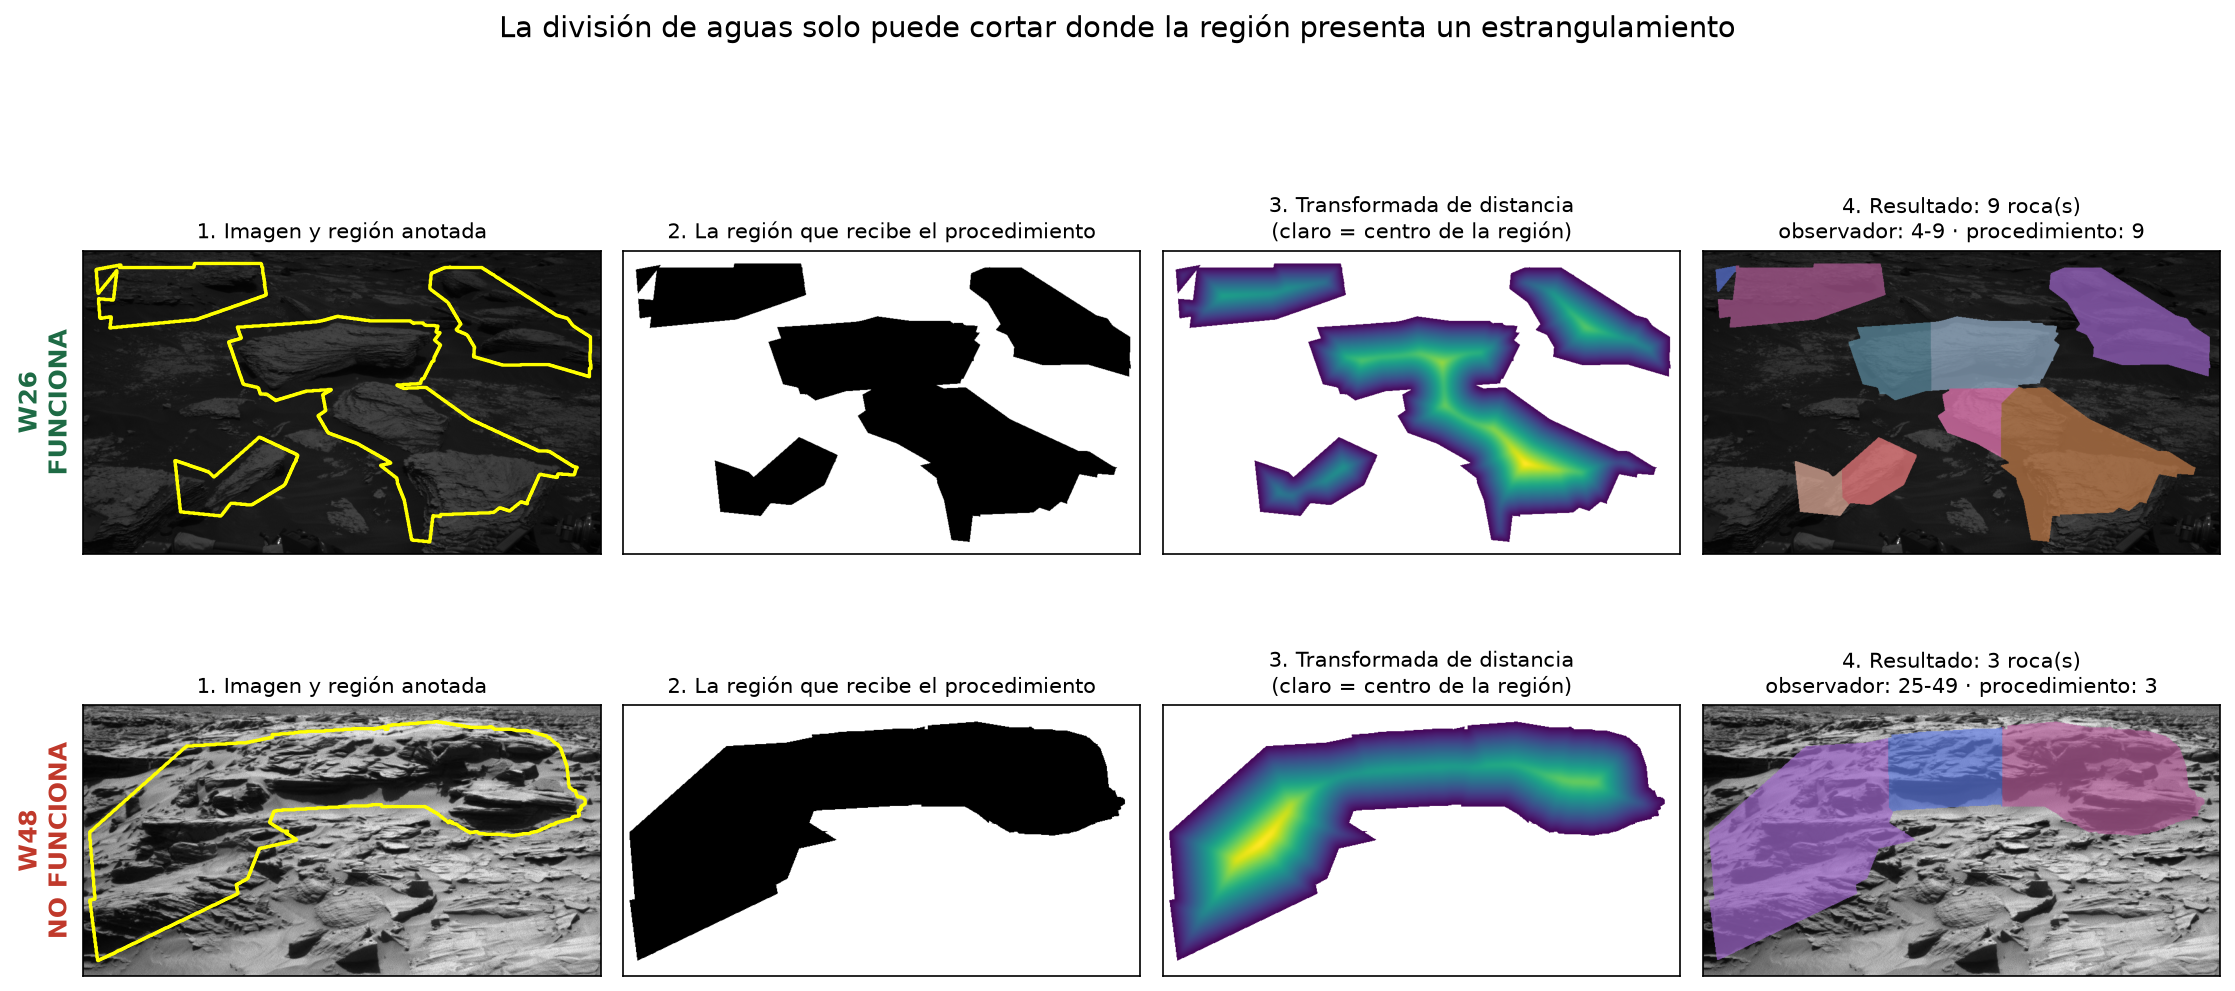
\includegraphics[width=\textwidth]{Figura_28_mecanismo_subconteo.png}
  \caption{Arriba, la anotación traza cada bloque por separado: hay regiones distintas con
    estrangulamientos claros y el corte funciona. Abajo, un único polígono trazado
    holgadamente sobre un campo de roca estratificada: la transformada de distancia forma
    una sola meseta y, por muchas rocas que contenga, no hay por dónde cortar.}
  \label{fig:mecanismo}
\end{figure}

La consecuencia, que el documento declara: el indicador \textbf{no estima el número de
rocas de una escena}, sino el de bloques dentro de la fracción que el anotador decidió
delimitar. Ambas cantidades pueden diferir en un orden de magnitud.

\subsection{Contraste con aprendizaje automático}

Se contrastó el procedimiento con dos enfoques, ejecutados en equipo local.

\textbf{Modelo general, sin entrenamiento específico.} Un modelo fundacional de
segmentación (FastSAM) aplicado a \num{50} escenas, restringido a la región de roca. El
acuerdo con el conteo clásico es del \SI{52}{\percent} por bandas, con correlación de
rangos de $0{,}45$ y error absoluto medio de $2{,}6$ rocas. Tiende a subdividir una misma
roca según su textura interna y a no detectar bloques de bajo contraste.

\textbf{Modelo entrenado con las propias máscaras.} Un segmentador DeepLabV3 por
aprendizaje por transferencia, que distingue roca de no-roca leyendo la imagen
\textbf{sin máscara humana}. Alcanza un IoU medio de $0{,}940$ y su cobertura correlaciona
$0{,}950$ con la humana.

\subsubsection*{Una hipótesis que hubo que poner a prueba}

Esa cifra de $0{,}940$ \textbf{no puede leerse como acierto}: el modelo se entrenó con
máscaras colaborativas y se evaluó contra máscaras colaborativas, de modo que mide cuánto
se parece a la anotación de la que aprendió. Y como esa anotación sobreestima la roca
(sección~\ref{sec:sesgo-doc}), lo esperable era que el modelo hubiera aprendido el sesgo
junto con la señal.

\begin{caja}
\noindent\textbf{La prueba.} Si el modelo heredó el sesgo, al evaluarlo contra las
\num{322} máscaras de experto debería \textbf{sobreestimar} la cobertura de forma
sistemática, igual que las máscaras con las que aprendió.

\smallskip
\noindent\textbf{El resultado.} No sobreestima. La mediana del error es de
$\mathbf{+0{,}0}$ \textbf{puntos porcentuales}, con un \SI{37}{\percent} de escenas por
encima y un \SI{30}{\percent} por debajo. \emph{La hipótesis queda descartada.}
\end{caja}

\begin{table}[H]
\centering\small
\begin{tabular}{lcc}
\toprule
\textbf{Medida} & \textbf{Contra colaborativas} & \textbf{Contra experto}\\
\midrule
IoU medio & 0,940 & 0,843\\
Correlación de la cobertura & 0,950 & 0,927\\
Error absoluto medio & 4,3 p.p. & 7,5 p.p.\\
Mediana del error (sesgo) & --- & \textbf{$+0{,}0$ p.p.}\\
\bottomrule
\end{tabular}
\caption{El desempeño baja al salir del dominio de entrenamiento, como era previsible,
  pero el modelo no arrastra el sesgo de la anotación.}
\end{table}

\begin{figure}[H]
  \centering
  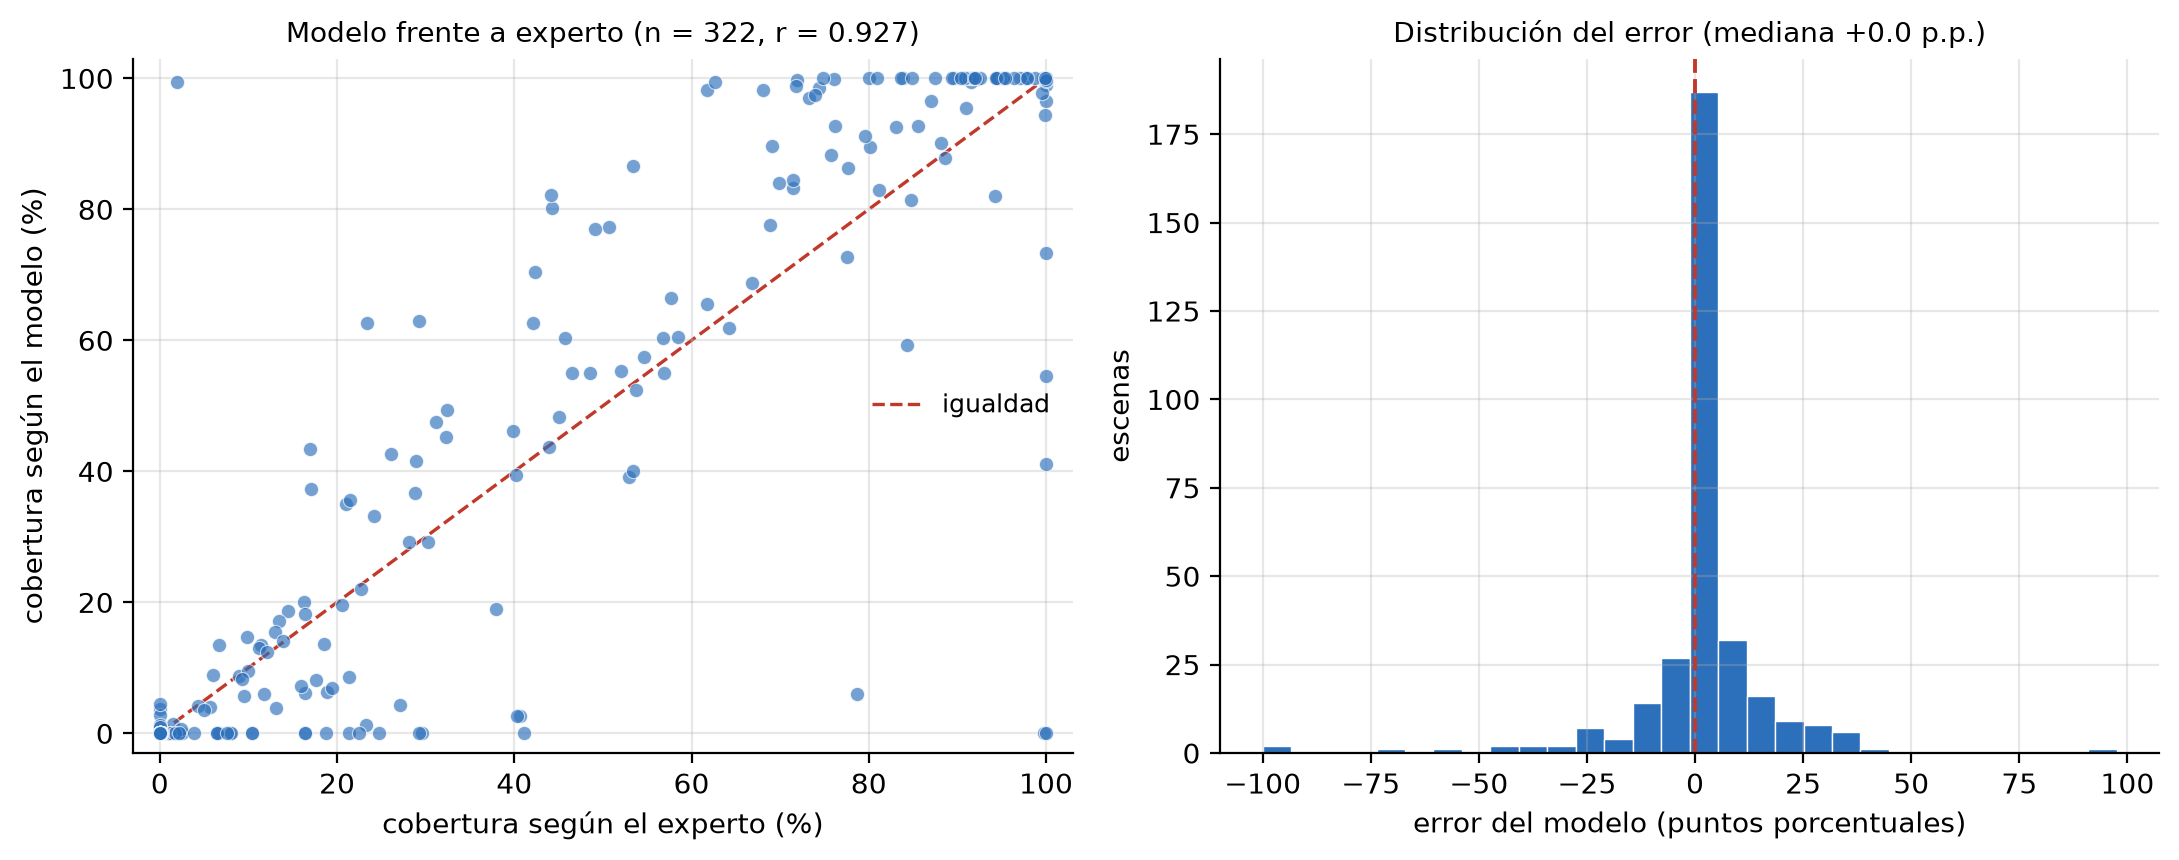
\includegraphics[width=\textwidth]{Figura_27_modelo_vs_experto.png}
  \caption{Izquierda: cobertura del modelo frente a la del experto; los puntos se reparten
    a ambos lados de la recta de igualdad. Derecha: el error se concentra en cero, sin
    desplazamiento hacia la sobreestimación.}
\end{figure}

\noindent\textbf{Por qué no lo heredó.} Encaja con el mecanismo del sesgo. Este opera por
el \textbf{denominador} —el suelo y la arena sin etiquetar, que salen del cálculo— y no por
error de clase en los píxeles que sí se etiquetan. Como el entrenamiento excluye los
píxeles sin etiqueta de la función de pérdida, el modelo aprendió apariencia de roca a
partir de píxeles correctamente etiquetados. \emph{El sesgo vivía en la fórmula de
agregación, no en el contenido de las etiquetas.}

\smallskip
\noindent\textbf{Reservas que declaro.} Estima \textbf{cobertura, no conteo}: no separa
bloques y no sustituye a E2. Y es fiable \textbf{en agregado, no escena por escena}: el
error absoluto medio es de $7{,}5$ puntos, el \SI{23}{\percent} de las escenas supera los
diez puntos y cinco superan los cincuenta.

\smallskip
\noindent\textbf{Lo que abre.} El procedimiento clásico necesita una máscara humana, que no
existe cuando las imágenes llegan a la Tierra. El segmentador lee la imagen directamente.
Que estime la cobertura sin sesgo frente a una referencia de experto sugiere que el
indicador definido y auditado aquí podría calcularse \textbf{sin anotación humana en el
bucle}.

\section{La extensión aplicada}

Los indicadores se tradujeron en seis reglas de aviso de terreno, con umbrales fijados
sobre percentiles de la distribución observada y cada uno acompañado de su justificación.
De las \num{16064} escenas, \num{104} resultan de riesgo alto y \num{1359} de riesgo medio.
Se desarrolló además una aplicación de escritorio con cuatro vistas para consultar los
resultados sin programar.

\begin{figure}[H]
  \centering
  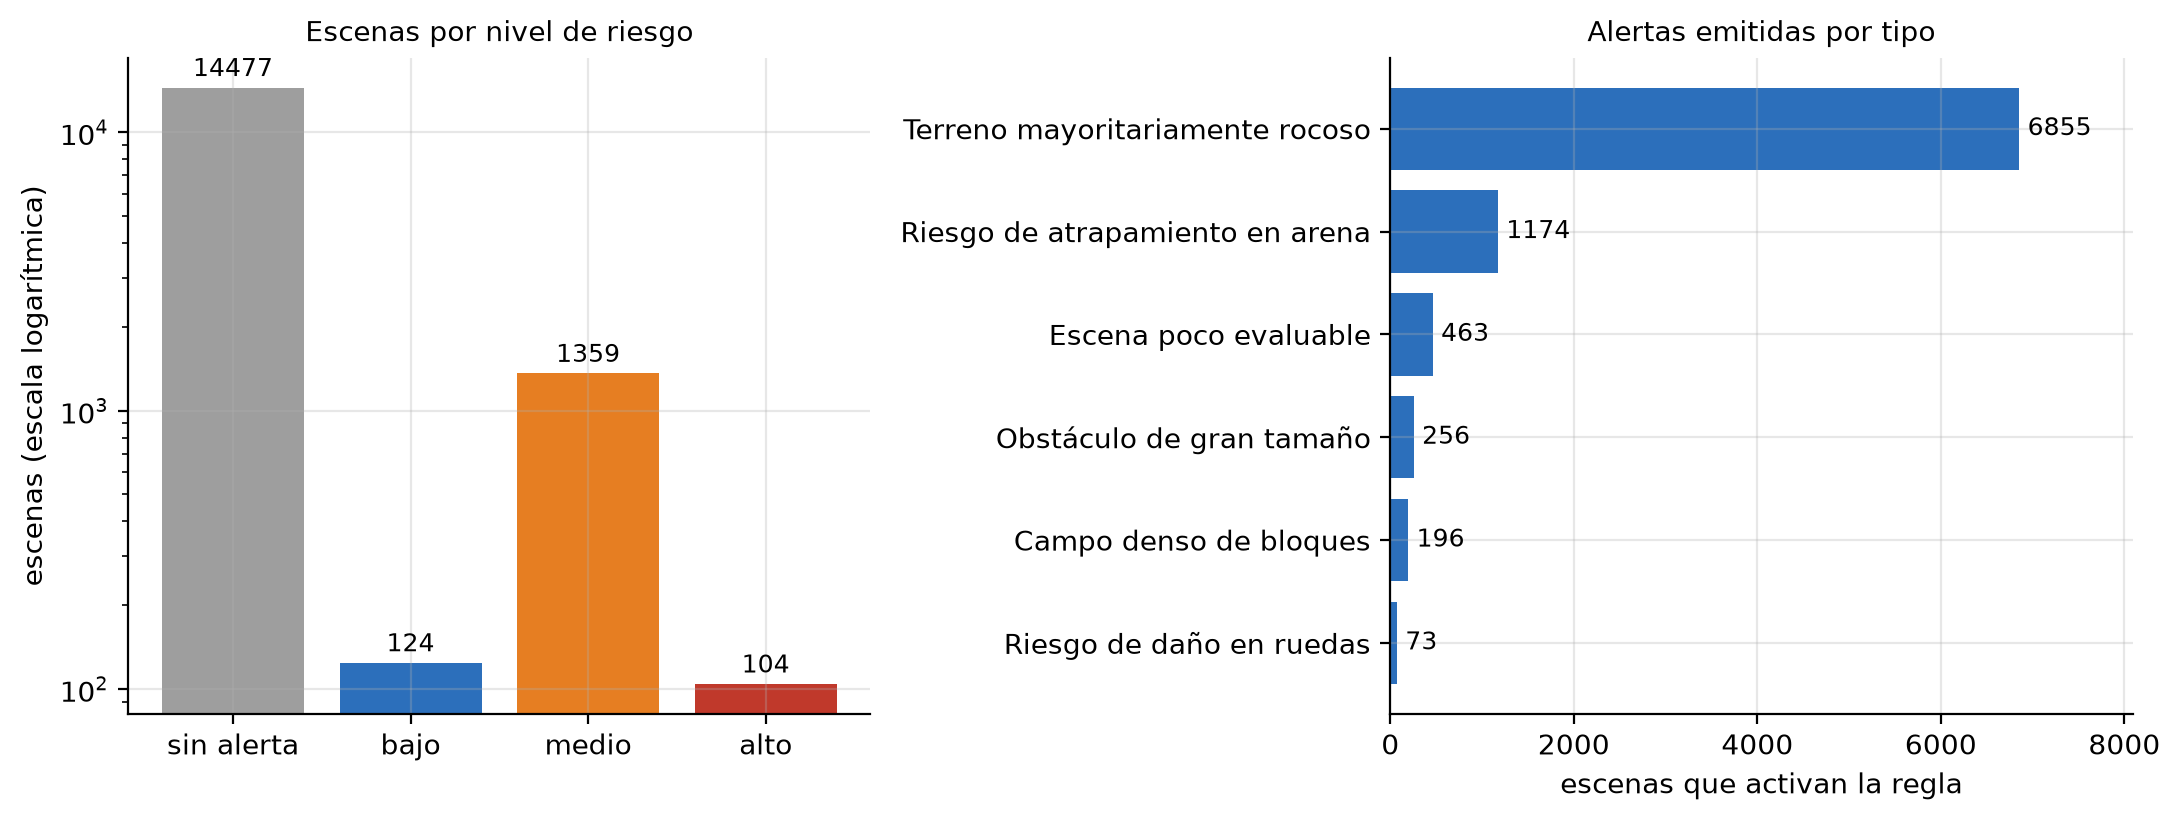
\includegraphics[width=\textwidth]{Figura_24_alertas_terreno.png}
  \caption{Escenas por nivel de riesgo y avisos emitidos por tipo.}
\end{figure}

\noindent\textbf{Cómo está presentado hoy:} como subsección del capítulo de resultados y
con la documentación técnica en anexo, \emph{no} como capítulo propio. El documento declara
que los avisos heredan las limitaciones de los indicadores de los que derivan y que no son
una valoración de transitabilidad validada contra incidentes reales.

\section{Preguntas y decisiones a consultar}
\label{sec:preguntas}

\preg{¿Autoriza un capítulo propio de «Desarrollo e implementación» para el sistema de
avisos y la aplicación?}
La plantilla lo omite por defecto en la modalidad de investigación, y solo lo admite «si la
investigación incluye el desarrollo e implementación de un artefacto sustantivo que
justifique un capítulo independiente, \textbf{con autorización del tutor}». Hoy está como
subsección de resultados. Si lo autoriza, el cambio es inmediato y el texto ya existe.

\preg{¿Le parece correcto que el aporte principal sea el diagnóstico del conjunto de datos
y no el indicador en sí?}
El trabajo responde su pregunta, pero lo que resultó más sólido y transferible fue el
hallazgo del sesgo de anotación y la atribución de los límites del conteo. Quiero
confirmar que ese encuadre es adecuado para la modalidad.

\preg{¿Cómo debo presentar los resultados negativos?}
Hay dos: la detección de vetas desde la imagen no es viable, y el conteo tiene un techo
estructural. Están reportados como resultados con su medición. ¿Es el tratamiento que
espera, o preferiría más peso en lo que sí funcionó?

\preg{La validación humana tiene un solo observador. ¿Es suficiente o debo ampliarla?}
Son \num{60} escenas con un observador. Está declarado como limitación. Ampliarla a varias
personas daría intervalos de confianza, pero requiere tiempo de terceros.

\preg{¿Incorporo al cuerpo el conteo híbrido (máscara + imagen)?}
Corrige el techo del conteo y elimina el sesgo, pero la mejora en acuerdo con el juicio
humano \textbf{no es estadísticamente demostrable} con \num{60} escenas (diferencia de
$+0{,}10$ en kappa ponderado, intervalo de confianza $[-0{,}12;\ +0{,}31]$). Mi inclinación
es dejarlo como línea futura y no en el cuerpo, para no tener que defender un resultado no
concluyente.

\preg{¿Amplío la justificación con el contexto operativo de las misiones?}
El documento no explica hoy \emph{por qué importa} explotar automáticamente la información
de terreno. Propongo dos o tres párrafos sobre el ciclo de comando de un rover —la latencia
de la señal y la planificación diaria— para dar ese «para qué», sin prometer que el
procedimiento opere en tiempo real, porque no puede.

\preg{¿Debo extender el alcance al conjunto de Perseverance?}
Su taxonomía geológica distingue \textbf{roca suelta}, presente en el \SI{63.8}{\percent} de
sus escenas frente al \SI{13.9}{\percent} de roca grande en el subconjunto actual. Es la vía
natural para sortear el techo del conteo, pero implica otro rover, otra cámara y otro sitio:
sería un segundo subconjunto, no más datos para los resultados actuales. Mi inclinación es
dejarlo como trabajo futuro.

\preg{Cuestiones de forma}
\begin{itemize}
  \item Su nombre completo, para la portada.
  \item ¿Debo activar las secciones opcionales de declaración y agradecimientos?
  \item Fechas de entrega y de sustentación, y si desea revisar por capítulos.
\end{itemize}

\section{Lo que haría a continuación}

\begin{enumerate}
  \item Aplicar lo que resulte de esta reunión.
  \item Ampliar la justificación con el contexto operativo (Pregunta~6).
  \item Compilar la versión definitiva en Overleaf, con la bibliografía en APA 7.
  \item Revisión final de redacción y coherencia de cifras.
\end{enumerate}

\end{document}
